\documentclass[11pt, a4paper]{article}

% Fonts and Encoding
\usepackage[utf8]{inputenc}
\usepackage[T1]{fontenc}
\usepackage{lmodern}\usepackage{lmodern}

% Math and Symbols
\usepackage{amsmath, amssymb, amsthm, amsfonts, mathrsfs, mathtools}

% Layout and Geometry
\usepackage{geometry}
\geometry{a4paper, margin=1in}

% Formatting and Graphics
\usepackage{graphicx, xcolor, enumitem, booktabs, array, tabularx}

% TikZ for Illustrations
\usepackage{tikz}
\usetikzlibrary{arrows.meta, positioning, shapes.geometric, calc, backgrounds, matrix}

% Clickable Links and TOC
\usepackage{hyperref}
\hypersetup{
    colorlinks=true,
    linkcolor=blue,
    filecolor=magenta,      
    urlcolor=cyan,
    pdftitle={Advanced Mathematics: Bijective Functions},
}

% Theorem Environments
\newtheorem{theorem}{Theorem}[section]
\newtheorem{lemma}[theorem]{Lemma}
\newtheorem{proposition}[theorem]{Proposition}
\newtheorem{corollary}[theorem]{Corollary}
\theoremstyle{definition}
\newtheorem{definition}{Definition}[section]
\newtheorem{axiom}{Axiom}[section]
\newtheorem{example}{Example}[section]
\theoremstyle{remark}
\newtheorem{remark}{Remark}[section]

% Custom Commands (Enforced standard notation)
\newcommand{\R}{\mathbb{R}}
\newcommand{\N}{\mathbb{N}}
\newcommand{\Z}{\mathbb{Z}}
\newcommand{\Q}{\mathbb{Q}}
\newcommand{\E}{\mathbb{E}}
\newcommand{\Prob}{\mathbb{P}}
\newcommand{\F}{\mathcal{F}}
\newcommand{\dom}{\operatorname{dom}}
\newcommand{\range}{\operatorname{range}}

\title{\textbf{Advanced Mathematics: Bijective Functions \\ \Large Foundations, Proofs, and Applications in Quantitative Modeling}}
\author{Tashfeen Omran}
\date{\today}

\begin{document}

\maketitle
\tableofcontents
\newpage

\section{Part 1: Comprehensive Introduction, Context, and Prerequisites}

\subsection{Core Concepts \& Axioms}
In the rigorous study of abstract mathematics, a function (or mapping) is not merely a computational formula, but a strictly defined relation between two sets. Let $A$ and $B$ be sets. A function $f: A \to B$ is a subset of the Cartesian product $A \times B$ such that for every $a \in A$, there exists exactly one $b \in B$ for which $(a, b) \in f$. We denote this as $f(a) = b$. The set $A$ is the \textit{domain}, and $B$ is the \textit{codomain}.

To understand the structural relationship between these sets, we classify functions based on how they map elements:
\begin{itemize}
    \item \textbf{Injective (One-to-One):} A function $f$ is injective if it never maps distinct elements of its domain to the same element of its codomain. Formally: $\forall x, y \in A, f(x) = f(y) \implies x = y$.
    \item \textbf{Surjective (Onto):} A function $f$ is surjective if its range equals its codomain. Every element in $B$ is "hit" by at least one element in $A$. Formally: $\forall y \in B, \exists x \in A \text{ such that } f(x) = y$.
    \item \textbf{Bijective (One-to-One Correspondence):} A function is bijective if it is both injective and surjective. A bijection establishes a perfect pairing between the elements of $A$ and $B$.
\end{itemize}

\subsection{Intuition and Set-Theoretic Foundations}
Intuitively, think of the domain $A$ as a set of "arrows" and the codomain $B$ as a set of "targets." 
A function requires that every arrow is shot exactly once. 
An \textit{injective} function guarantees that no two arrows hit the same target. 
A \textit{surjective} function guarantees that every target is hit by at least one arrow. 
A \textit{bijective} function means there is exactly one arrow for every target, implying that the sets $A$ and $B$ have the exact same "size" or \textit{cardinality}. In set theory, two sets $A$ and $B$ are defined to have the same cardinality ($|A| = |B|$) if and only if there exists a bijection $f: A \to B$.

\subsection{Historical Context and Motivation}
The formalization of functions and bijections was driven by the foundational crisis of mathematics in the late 19th century, spearheaded by Georg Cantor. Before Cantor, infinity was treated as a singular, vague concept. By using bijections, Cantor rigorously proved that there are different "sizes" of infinity. For instance, he showed that there exists a bijection between the natural numbers $\N$ and the rational numbers $\Q$, but no bijection can exist between $\N$ and the real numbers $\R$ (Cantor's Diagonal Argument). This revolutionized set theory, topology, and modern probability theory, where measure spaces rely heavily on the cardinality of sets.

\subsection{Key Theorems, Lemmas, and Formulas}
\begin{theorem}[Permutations of Finite Sets]
If $A$ and $B$ are finite sets with $|A| = |B| = n$, then there are exactly $n!$ bijective functions from $A$ to $B$.
\end{theorem}

\begin{theorem}[Finiteness and Bijections]
Let $A$ and $B$ be finite nonempty sets such that $|A| = |B|$, and let $f: A \to B$ be a function. Then $f$ is injective if and only if $f$ is surjective. (Note: This fails for infinite sets).
\end{theorem}

\subsection{Prerequisites}
To master this chapter, the reader must be proficient in:
\begin{enumerate}
    \item \textbf{Direct Proofs and Contradiction:} Setting up $f(a) = f(b)$ and algebraically deducing $a = b$.
    \item \textbf{Modular Arithmetic:} Understanding equivalence classes (e.g., $\Z_n$) to prove functions are well-defined.
    \item \textbf{Basic Set Theory:} Intersections, unions, subsets, and Cartesian products.
\end{enumerate}

\newpage
\section{Part 2: Detailed Homework Solutions}

\subsection{Problem 10.20}
\textbf{Problem:} A function $f: \Z \to \Z$ is defined by $f(n) = 2n + 1$. Determine whether $f$ is (a) injective, (b) surjective.

\textbf{Solution:}
\begin{proof}[Proof of (a) Injectivity]
We use a direct proof. Let $a, b \in \Z$ and assume $f(a) = f(b)$. 
\[ 2a + 1 = 2b + 1 \]
Subtracting $1$ from both sides yields $2a = 2b$. Dividing by $2$ yields $a = b$. 
Since $f(a) = f(b) \implies a = b$, the function $f$ is \textbf{injective}.
\end{proof}

\begin{proof}[Proof of (b) Surjectivity]
We use a proof by counterexample. For $f$ to be surjective, for every $y \in \Z$, there must exist an $n \in \Z$ such that $f(n) = y$. 
Let $y = 2 \in \Z$. We set up the equation:
\[ 2n + 1 = 2 \implies 2n = 1 \implies n = \frac{1}{2} \]
Since $\frac{1}{2} \notin \Z$, there is no integer $n$ that maps to $2$. Thus, $f$ is \textbf{not surjective}.
\end{proof}

\subsection{Problem 10.21}
\textbf{Problem:} A function $f: \Z \to \Z$ is defined by $f(n) = n - 3$. Determine whether $f$ is (a) injective, (b) surjective.

\textbf{Solution:}
\begin{proof}[Proof of (a) Injectivity]
Let $a, b \in \Z$ and assume $f(a) = f(b)$. 
\[ a - 3 = b - 3 \]
Adding $3$ to both sides yields $a = b$. Thus, $f$ is \textbf{injective}.
\end{proof}

\begin{proof}[Proof of (b) Surjectivity]
Let $y \in \Z$ be an arbitrary integer in the codomain. We must find an $n \in \Z$ such that $f(n) = y$.
\[ n - 3 = y \implies n = y + 3 \]
Since the integers are closed under addition, $y + 3 \in \Z$. Furthermore, $f(y+3) = (y+3) - 3 = y$. Thus, $f$ is \textbf{surjective}.
\end{proof}

\subsection{Problem 10.22}
\textbf{Problem:} A function $f: \Z \to \Z$ is defined by $f(n) = 5n + 2$. Determine whether $f$ is (a) injective, (b) surjective.

\textbf{Solution:}
\begin{proof}[Proof of (a) Injectivity]
Let $a, b \in \Z$ and assume $f(a) = f(b)$. 
\[ 5a + 2 = 5b + 2 \implies 5a = 5b \implies a = b \]
Thus, $f$ is \textbf{injective}.
\end{proof}

\begin{proof}[Proof of (b) Surjectivity]
Let $y = 3 \in \Z$. We require $n \in \Z$ such that $5n + 2 = 3$.
\[ 5n = 1 \implies n = \frac{1}{5} \]
Since $\frac{1}{5} \notin \Z$, $3$ has no pre-image. Thus, $f$ is \textbf{not surjective}.
\end{proof}

\subsection{Problem 10.23}
\textbf{Problem:} Prove or disprove: For every nonempty set $A$, there exists an injective function $f: A \to \mathcal{P}(A)$.

\textbf{Solution:}
\begin{proof}
The statement is \textbf{True}. We provide a direct proof by constructing such a function.
Let $A$ be an arbitrary nonempty set. Define $f: A \to \mathcal{P}(A)$ by $f(x) = \{x\}$ for all $x \in A$. 
Since $x \in A$, the singleton set $\{x\}$ is a subset of $A$, meaning $\{x\} \in \mathcal{P}(A)$. Thus, the codomain is correct.
To show injectivity, let $a, b \in A$ and assume $f(a) = f(b)$. 
\[ \{a\} = \{b\} \]
By the axiom of extensionality in set theory, two sets are equal if and only if they contain the exact same elements. Therefore, the single element in the first set must equal the single element in the second set, yielding $a = b$. 
Thus, $f$ is injective.
\end{proof}

\subsection{Problem 10.24}
\textbf{Problem:} Determine whether the function $f: \R \to \R$ defined by $f(x) = x^2 + 4x + 9$ is (a) one-to-one, (b) onto.

\textbf{Solution:}
First, we complete the square for $f(x)$:
\[ f(x) = (x^2 + 4x + 4) + 5 = (x+2)^2 + 5 \]
\begin{proof}[Proof of (a) One-to-One]
Let $x_1 = -1$ and $x_2 = -3$. 
$f(-1) = (-1+2)^2 + 5 = 1 + 5 = 6$.
$f(-3) = (-3+2)^2 + 5 = 1 + 5 = 6$.
Since $f(-1) = f(-3)$ but $-1 \neq -3$, $f$ is \textbf{not one-to-one}.
\end{proof}

\begin{proof}[Proof of (b) Onto]
Notice that for any $x \in \R$, $(x+2)^2 \ge 0$. Therefore, $f(x) = (x+2)^2 + 5 \ge 5$. 
Let $y = 0 \in \R$ (the codomain). There is no real number $x$ such that $f(x) = 0$, because $f(x) \ge 5$ for all $x \in \R$. Thus, $f$ is \textbf{not onto}.
\end{proof}

\subsection{Problem 10.25}
\textbf{Problem:} Is there a function $f: \R \to \R$ that is onto but not one-to-one? Explain your answer.

\textbf{Solution:}
\textbf{Yes.} Consider the cubic function $f(x) = x^3 - x$. 
\begin{itemize}
    \item \textbf{Not one-to-one:} Observe that $f(0) = 0^3 - 0 = 0$, $f(1) = 1^3 - 1 = 0$, and $f(-1) = (-1)^3 - (-1) = 0$. Since multiple distinct inputs map to $0$, $f$ is not injective.
    \item \textbf{Onto:} $f(x)$ is a continuous polynomial of odd degree. As $x \to \infty$, $f(x) \to \infty$, and as $x \to -\infty$, $f(x) \to -\infty$. By the Intermediate Value Theorem, $f(x)$ takes on all real values. Thus, $f$ is surjective.
\end{itemize}

\subsection{Problem 10.26}
\textbf{Problem:} Give an example of a function $f: \N \to \N$ that is (a) one-to-one and onto, (b) one-to-one but not onto, (c) onto but not one-to-one, (d) neither one-to-one nor onto.

\textbf{Solution:}
\begin{enumerate}[label=(\a)]
    \item \textbf{One-to-one and onto:} The identity function $f(n) = n$.
    \item \textbf{One-to-one but not onto:} $f(n) = n + 1$. (It is injective since $a+1=b+1 \implies a=b$. It is not onto because $1 \in \N$ has no pre-image in $\N$).
    \item \textbf{Onto but not one-to-one:} 
    \[
    f(n) = \begin{cases} 
      1 & \text{if } n = 1 \\
      n - 1 & \text{if } n \ge 2 
   \end{cases}
    \]
    (It is onto because for any $y \in \N$, $f(y+1) = y$. It is not one-to-one because $f(1) = 1$ and $f(2) = 1$).
    \item \textbf{Neither:} $f(n) = 1$ for all $n \in \N$. (Not injective since $f(1)=f(2)=1$. Not onto since $2$ has no pre-image).
\end{enumerate}

\subsection{Problem 10.27}
\textbf{Problem:} Let $A = \{2, 3, 4, 5\}$ and $B = \{6, 8, 10\}$. A relation $R$ is defined from $A$ to $B$ by $aRb$ if $a \mid b$ and $(b/a) + 1$ is a prime. (a) Is $R$ a function from $A$ to $B$? (b) If $R$ is a function, determine whether it is one-to-one and/or onto.

\textbf{Solution:}
First, we explicitly determine the elements of $R$ by testing all pairs $(a,b) \in A \times B$:
\begin{itemize}
    \item $a=2$: $2|6 \implies 6/2+1=4$ (not prime). $2|8 \implies 8/2+1=5$ (prime). $2|10 \implies 10/2+1=6$ (not prime). $\implies (2,8) \in R$.
    \item $a=3$: $3|6 \implies 6/3+1=3$ (prime). $3 \nmid 8$. $3 \nmid 10$. $\implies (3,6) \in R$.
    \item $a=4$: $4 \nmid 6$. $4|8 \implies 8/4+1=3$ (prime). $4 \nmid 10$. $\implies (4,8) \in R$.
    \item $a=5$: $5 \nmid 6$. $5 \nmid 8$. $5|10 \implies 10/5+1=3$ (prime). $\implies (5,10) \in R$.
\end{itemize}
Thus, $R = \{(2,8), (3,6), (4,8), (5,10)\}$.

\begin{proof}[Answer to (a)]
Yes, $R$ is a function. Every element $a \in A$ appears exactly once as the first coordinate in the ordered pairs of $R$.
\end{proof}

\begin{proof}[Answer to (b)]
\textbf{Not one-to-one:} $R(2) = 8$ and $R(4) = 8$. Since $2 \neq 4$, it is not injective. \\
\textbf{Onto:} The range of $R$ is $\{6, 8, 10\}$, which exactly equals the codomain $B$. Thus, it is surjective.
\end{proof}

\subsection{Problem 10.28}
\textbf{Problem:} Let $A = \{2, 4, 6\}$ and $B = \{1, 3, 4, 7, 9\}$. A relation $f$ is defined from $A$ to $B$ by $afb$ if $5 \mid (ab + 1)$. Is $f$ a one-to-one function?

\textbf{Solution:}
Let us find the pairs $(a,b)$ that satisfy $ab + 1 \equiv 0 \pmod 5$, which means $ab \equiv 4 \pmod 5$.
\begin{itemize}
    \item $a=2$: $2b \equiv 4 \pmod 5 \implies b \equiv 2 \pmod 5$. In $B$, the only element is $b=7$. So $(2,7) \in f$.
    \item $a=4$: $4b \equiv 4 \pmod 5 \implies b \equiv 1 \pmod 5$. In $B$, the only element is $b=1$. So $(4,1) \in f$.
    \item $a=6$: $6 \equiv 1 \pmod 5$, so $1 \cdot b \equiv 4 \pmod 5 \implies b \equiv 4 \pmod 5$. In $B$, the elements satisfying this are $b=4$ and $b=9$. So $(6,4) \in f$ and $(6,9) \in f$.
\end{itemize}
Since the element $6 \in A$ maps to two distinct elements in $B$ ($4$ and $9$), $f$ is \textbf{not a function}. Consequently, it cannot be a one-to-one function.

\subsection{Problem 10.29}
\textbf{Problem:} Let $f$ be a function with $\dom(f) = A$ and let $C$ and $D$ be subsets of $A$. Prove that if $f$ is one-to-one, then $f(C \cap D) = f(C) \cap f(D)$.

\textbf{Solution:}
\begin{proof}
We must prove two subset inclusions. \\
\textbf{Part 1: $f(C \cap D) \subseteq f(C) \cap f(D)$} (This holds for all functions). \\
Let $y \in f(C \cap D)$. By definition, there exists $x \in C \cap D$ such that $f(x) = y$. 
Since $x \in C \cap D$, we know $x \in C$ and $x \in D$. 
Because $x \in C$, $f(x) \in f(C)$. Because $x \in D$, $f(x) \in f(D)$. 
Therefore, $y = f(x) \in f(C) \cap f(D)$.

\textbf{Part 2: $f(C) \cap f(D) \subseteq f(C \cap D)$} (This requires $f$ to be one-to-one). \\
Let $y \in f(C) \cap f(D)$. This means $y \in f(C)$ and $y \in f(D)$. 
Since $y \in f(C)$, there exists $c \in C$ such that $f(c) = y$. 
Since $y \in f(D)$, there exists $d \in D$ such that $f(d) = y$. 
Thus, $f(c) = f(d)$. Because $f$ is given to be one-to-one, $f(c) = f(d) \implies c = d$. 
Let $x = c = d$. Since $x = c$, $x \in C$. Since $x = d$, $x \in D$. 
Therefore, $x \in C \cap D$. Since $y = f(x)$, we conclude $y \in f(C \cap D)$. 

Since both subset inclusions hold, $f(C \cap D) = f(C) \cap f(D)$.
\end{proof}

\subsection{Problem 10.30}
\textbf{Problem:} Prove that the function $f: \R \to \R$ defined by $f(x) = 7x - 2$ is bijective.

\textbf{Solution:}
\begin{proof}
\textbf{Injectivity:} Let $a, b \in \R$ and assume $f(a) = f(b)$. 
\[ 7a - 2 = 7b - 2 \implies 7a = 7b \implies a = b \]
Thus, $f$ is injective. \\
\textbf{Surjectivity:} Let $y \in \R$. We must find $x \in \R$ such that $f(x) = y$. 
\[ 7x - 2 = y \implies 7x = y + 2 \implies x = \frac{y + 2}{7} \]
Since $y \in \R$, $x = \frac{y+2}{7} \in \R$. Furthermore, $f\left(\frac{y+2}{7}\right) = 7\left(\frac{y+2}{7}\right) - 2 = y + 2 - 2 = y$. 
Thus, $f$ is surjective. Since $f$ is both injective and surjective, it is bijective.
\end{proof}

\subsection{Problem 10.31}
\textbf{Problem:} Let $f: \Z_5 \to \Z_5$ be a function defined by $f([a]) = [2a + 3]$. (a) Show that $f$ is well-defined. (b) Determine whether $f$ is bijective.

\textbf{Solution:}
\begin{proof}[Proof of (a) Well-defined]
To show $f$ is well-defined, we must prove that if $[a] = [b]$, then $f([a]) = f([b])$. 
Assume $[a] = [b]$. This means $a \equiv b \pmod 5$, so $a - b = 5k$ for some $k \in \Z$. 
We evaluate $f([a]) - f([b])$ internally:
\[ (2a + 3) - (2b + 3) = 2a - 2b = 2(a - b) = 2(5k) = 5(2k) \]
Since $5(2k)$ is a multiple of $5$, $(2a+3) \equiv (2b+3) \pmod 5$. Thus, $[2a+3] = [2b+3]$, meaning $f([a]) = f([b])$. The function is well-defined.
\end{proof}

\begin{proof}[Proof of (b) Bijective]
Since $\Z_5$ is a finite set and the domain and codomain have the same cardinality ($|\Z_5| = 5$), by Theorem 10.8, we only need to prove injectivity to establish bijectivity.
Assume $f([a]) = f([b])$. 
\[ [2a + 3] = [2b + 3] \implies 2a + 3 \equiv 2b + 3 \pmod 5 \implies 2a \equiv 2b \pmod 5 \]
Since $\gcd(2, 5) = 1$, we can multiply both sides by the modular inverse of $2$ (which is $3$) to cancel the $2$:
\[ 3(2a) \equiv 3(2b) \pmod 5 \implies 6a \equiv 6b \pmod 5 \implies a \equiv b \pmod 5 \]
Thus, $[a] = [b]$. $f$ is injective, and therefore bijective.
\end{proof}

\subsection{Problem 10.32}
\textbf{Problem:} Prove that the function $f: \R - \{2\} \to \R - \{5\}$ defined by $f(x) = \frac{5x+1}{x-2}$ is bijective.

\textbf{Solution:}
\begin{proof}
\textbf{Injectivity:} Let $a, b \in \R - \{2\}$ and assume $f(a) = f(b)$.
\[ \frac{5a+1}{a-2} = \frac{5b+1}{b-2} \]
Cross-multiplying yields:
\[ (5a+1)(b-2) = (5b+1)(a-2) \]
\[ 5ab - 10a + b - 2 = 5ab - 10b + a - 2 \]
Subtracting $5ab - 2$ from both sides:
\[ -10a + b = -10b + a \implies -11a = -11b \implies a = b \]
Thus, $f$ is injective.

\textbf{Surjectivity:} Let $y \in \R - \{5\}$. We must find $x \in \R - \{2\}$ such that $f(x) = y$.
\[ y = \frac{5x+1}{x-2} \implies y(x-2) = 5x+1 \implies yx - 2y = 5x + 1 \]
\[ yx - 5x = 2y + 1 \implies x(y - 5) = 2y + 1 \implies x = \frac{2y+1}{y-5} \]
Since $y \neq 5$, $x$ is a well-defined real number. We must also verify that $x \neq 2$. Suppose for contradiction that $x = 2$. Then:
\[ 2 = \frac{2y+1}{y-5} \implies 2(y-5) = 2y+1 \implies 2y - 10 = 2y + 1 \implies -10 = 1 \]
This is a contradiction. Thus, $x \in \R - \{2\}$. Since we found a valid pre-image for every $y$, $f$ is surjective. 
Being both injective and surjective, $f$ is bijective.
\end{proof}

\subsection{Problem 10.33}
\textbf{Problem:} Let $A = [0, 1]$. Give an example of two different bijective functions $f_1$ and $f_2$ from $A$ to $A$, neither of which is the identity function.

\textbf{Solution:}
\begin{enumerate}
    \item $f_1(x) = 1 - x$. (This reflects the interval $[0,1]$ across $x=0.5$. It is its own inverse, hence bijective).
    \item $f_2(x) = x^2$. (Since $x \ge 0$, $x^2$ is strictly increasing, making it injective. $f_2(0)=0$ and $f_2(1)=1$, and it is continuous, so by IVT it covers $[0,1]$, making it surjective).
\end{enumerate}

\subsection{Problem 10.34}
\textbf{Problem:} Give a proof of Theorem 10.7 using mathematical induction. (Theorem 10.7: If $A$ and $B$ are finite sets with $|A|=|B|=n$, there are $n!$ bijective functions from $A$ to $B$).

\textbf{Solution:}
\begin{proof}
We proceed by induction on $n$. \\
\textbf{Base Case ($n=1$):} Let $|A| = |B| = 1$. Let $A = \{a_1\}$ and $B = \{b_1\}$. There is exactly $1$ function from $A$ to $B$, defined by $f(a_1) = b_1$. This function is clearly bijective. Since $1! = 1$, the base case holds. \\
\textbf{Inductive Step:} Assume the theorem holds for some arbitrary integer $k \ge 1$. That is, for any sets of size $k$, there are $k!$ bijections between them. 
We must show it holds for $k+1$. Let $A$ and $B$ be sets such that $|A| = |B| = k+1$. 
Let $A = \{a_1, a_2, \dots, a_{k+1}\}$. 
To construct a bijection $f: A \to B$, we first choose an image for $a_{k+1}$. Since $|B| = k+1$, there are exactly $k+1$ choices for $f(a_{k+1})$. 
Suppose we choose $f(a_{k+1}) = b^* \in B$. For $f$ to be a bijection, the remaining elements of $A$ (which form a set $A' = A \setminus \{a_{k+1}\}$ of size $k$) must map bijectively to the remaining elements of $B$ (which form a set $B' = B \setminus \{b^*\}$ of size $k$). 
By the inductive hypothesis, there are exactly $k!$ such bijections from $A'$ to $B'$. 
Since there were $k+1$ independent choices for $f(a_{k+1})$, the total number of bijections from $A$ to $B$ is:
\[ (k+1) \times k! = (k+1)! \]
By the Principle of Mathematical Induction, the theorem holds for all $n \ge 1$.
\end{proof}

\subsection{Problem 10.35}
\textbf{Problem:} Domination number $\gamma(R)$ is the smallest cardinality of $S \subseteq A$ such that every $y \in B$ is related to by some $x \in S$.
(a) Determine $\gamma(R)$ for the given specific relation.
(b) If $R$ is an equivalence relation on $A$, what is $\gamma(R)$?
(c) If $f$ is a bijective function from $A$ to $B$, what is $\gamma(f)$?

\textbf{Solution:}
\begin{enumerate}[label=(\alph*)]
    \item \textbf{Given:} $A=\{1..7\}$, $B=\{a..g\}$. $R = \{(1,c), (1,e), (2,c), (2,f), (2,g), (3,b), (3,f), (4,a), (4,c), (4,g), (5,a), (5,b), (5,c), (6,d), (6,e), (7,a), (7,g)\}$. \\
    We need to cover $B = \{a,b,c,d,e,f,g\}$. 
    Notice $d \in B$ is only related to by $6 \in A$. Thus, $6$ \textbf{must} be in $S$. Element $6$ covers $\{d, e\}$. 
    Remaining to cover: $\{a, b, c, f, g\}$. 
    Element $3$ covers $\{b, f\}$. Remaining: $\{a, c, g\}$. 
    Element $4$ covers $\{a, c, g\}$. 
    Thus, $S = \{3, 4, 6\}$ covers all of $B$. $|S| = 3$. 
    Can we do it with 2 elements? Element $6$ is mandatory and covers 2 elements. We would need 1 more element to cover the remaining 5 elements of $B$. However, the maximum out-degree of any element in $A$ is 3. Thus, 1 element can cover at most 3 targets. We cannot cover 5 targets with 1 element. Therefore, the minimum size is 3. $\gamma(R) = 3$.
    
    \item \textbf{Equivalence Relation:} An equivalence relation partitions $A$ into disjoint equivalence classes. Elements in one class only relate to elements in that same class. To cover all elements of $A$ (since $B=A$), we must select at least one representative from every equivalence class. Thus, $\gamma(R)$ is exactly the \textbf{number of distinct equivalence classes} of $A$ under $R$.
    
    \item \textbf{Bijective Function:} A bijection $f: A \to B$ maps each element of $A$ to exactly one unique element of $B$. To cover all $|B|$ elements of $B$, we must use exactly $|B|$ elements of $A$. Since $|A| = |B|$, we must use every element of $A$. Thus, $\gamma(f) = |A|$.
\end{enumerate}

\subsection{Problem 10.36}
\textbf{Problem:} List functions $\phi: A \to B$ such that $\phi(r) \in L(r)$. 
(a) Does there exist a bijective list function for the first set of lists?
(b) Does there exist a bijective list function for the second set of lists?

\textbf{Solution:}
\begin{enumerate}[label=(\alph*)]
    \item $L(a)=\{w,x,y\}, L(b)=\{u,z\}, L(c)=\{u,v\}, L(d)=\{u,w\}, L(e)=\{u,x,y\}, L(f)=\{v,y\}$. \\
    \textbf{Yes.} We can construct one via logical deduction:
    Notice $z$ only appears in $L(b)$. So we must set $\phi(b) = z$. 
    Now $L(d) = \{u,w\}$. Let's set $\phi(d) = u$. 
    Then $L(c) = \{u,v\}$ must use $v$ (since $u$ is taken). $\phi(c) = v$. 
    Then $L(f) = \{v,y\}$ must use $y$ (since $v$ is taken). $\phi(f) = y$. 
    Then $L(e) = \{u,x,y\}$ must use $x$ (since $u, y$ are taken). $\phi(e) = x$. 
    Then $L(a) = \{w,x,y\}$ must use $w$ (since $x, y$ are taken). $\phi(a) = w$. 
    The mapping $\phi = \{(a,w), (b,z), (c,v), (d,u), (e,x), (f,y)\}$ is a valid bijection.
    
    \item $L(a)=\{u,v,x,y\}, L(b)=\{v,w,y\}, L(c)=\{v,y\}, L(d)=\{u,w,x,z\}, L(e)=\{v,w\}, L(f)=\{w,y\}$. \\
    \textbf{No.} Consider the subset of domain elements $S = \{b, c, e, f\}$. 
    The union of their allowed lists is $L(S) = L(b) \cup L(c) \cup L(e) \cup L(f) = \{v,w,y\} \cup \{v,y\} \cup \{v,w\} \cup \{w,y\} = \{v, w, y\}$. 
    We have $|S| = 4$ elements that must be mapped to distinct targets, but there are only $|L(S)| = 3$ available targets for them. By the Pigeonhole Principle (or Hall's Marriage Theorem), it is impossible to form an injective (and thus bijective) function.
\end{enumerate}

\newpage
\section{Part 3: In-Depth Analysis of Problems and Techniques}

\subsection{A) Problem Types and Logical Strategies}
\begin{itemize}
    \item \textbf{Algebraic Bijections (10.20-10.22, 10.24, 10.30-10.32):} These problems require standard algebraic manipulation. The strategy for injectivity is universally to assume $f(a) = f(b)$ and isolate variables to show $a=b$. The strategy for surjectivity is to set $f(x) = y$ and solve for $x$ in terms of $y$, then verify that the resulting $x$ is strictly within the defined domain.
    \item \textbf{Set-Theoretic/Abstract Proofs (10.23, 10.29):} These require element-chasing. To prove set equality $X = Y$, one must prove $X \subseteq Y$ and $Y \subseteq X$ by taking an arbitrary element $x \in X$ and logically deducing $x \in Y$.
    \item \textbf{Combinatorial/Graph-Theoretic (10.35, 10.36):} These problems introduce concepts from graph theory (Domination Number) and combinatorics (System of Distinct Representatives). The strategy relies on extreme cases, Pigeonhole Principle, and Hall's Marriage Condition.
\end{itemize}

\subsection{B) Key Analytical and Logical Manipulations}
\begin{itemize}
    \item \textbf{Completing the Square (10.24):} A critical algebraic trick to analyze quadratic functions. By writing $x^2 + 4x + 9$ as $(x+2)^2 + 5$, the lower bound becomes immediately obvious, instantly disproving surjectivity.
    \item \textbf{Modular Arithmetic Cancellation (10.31):} When proving injectivity in $\Z_n$, one cannot simply divide. The logical manipulation requires multiplying by the modular inverse. In $\Z_5$, to solve $2a \equiv 2b \pmod 5$, we multiply by $3$ (since $3 \times 2 = 6 \equiv 1 \pmod 5$) to isolate $a \equiv b$.
    \item \textbf{Hall's Marriage Condition (10.36b):} To prove a bijection \textit{cannot} exist in a bipartite matching scenario, the most elegant trick is to find a subset of domain elements $S$ whose collective target list $L(S)$ is strictly smaller than $|S|$.
\end{itemize}

\newpage
\section{Part 4: "Cheatsheet", Visuals, and Tips for Success}

\subsection{Theorems \& Equivalences}
\renewcommand{\arraystretch}{1.5}
\begin{table}[h!]
\centering
\begin{tabularx}{\textwidth}{>{\raggedright\arraybackslash}p{4cm} X}
\toprule
\textbf{Concept} & \textbf{Formal Definition / Equivalence} \\
\midrule
\textbf{Injectivity (1-to-1)} & $f(a) = f(b) \implies a = b$. Equivalently (contrapositive): $a \neq b \implies f(a) \neq f(b)$. \\
\textbf{Surjectivity (Onto)} & $\forall y \in B, \exists x \in A \text{ s.t. } f(x) = y$. Equivalently: $\range(f) = \text{codomain}(f)$. \\
\textbf{Bijectivity} & $f$ is both injective and surjective. Equivalently: $f$ has a well-defined two-sided inverse $f^{-1}$. \\
\textbf{Finite Set Cardinality} & If $|A| = |B| < \infty$, then $f: A \to B$ is injective $\iff$ $f$ is surjective. \\
\bottomrule
\end{tabularx}
\end{table}

\subsection{Set \& Logic Illustrations: Bijective Mapping}
The following TikZ diagram illustrates a perfect bijective mapping between two sets, $A$ and $B$. Notice how every node in $A$ has exactly one outgoing arrow, and every node in $B$ has exactly one incoming arrow.

\vspace{1em}
\begin{center}
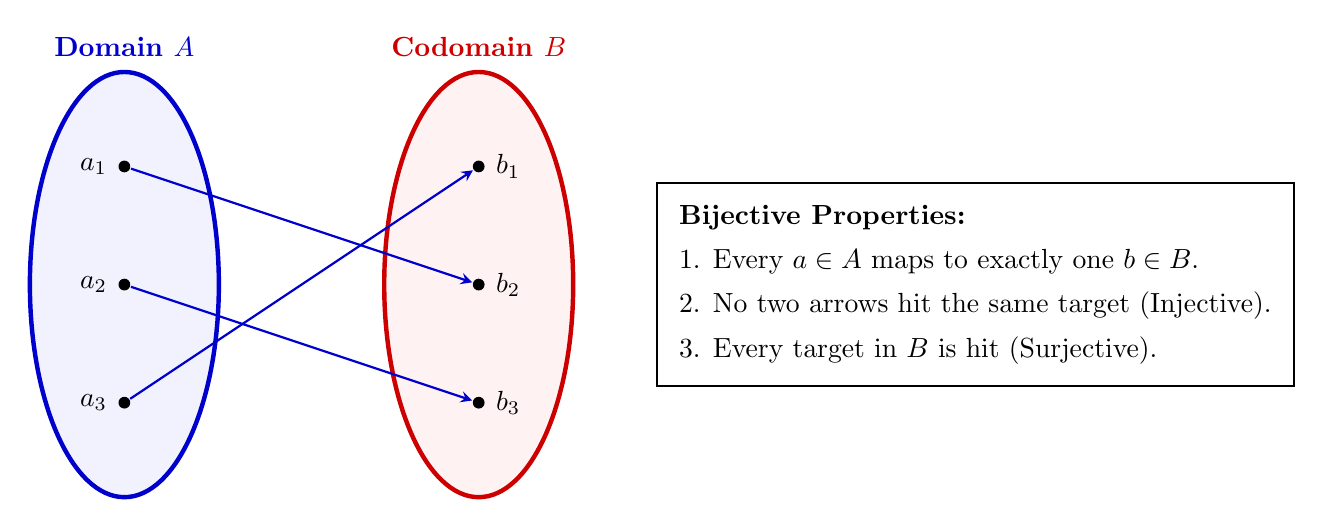
\begin{tikzpicture}[scale=1.5, >=stealth, thick]
    % Background fills for sets
    \fill[blue!5] (-1, 1.5) ellipse (0.8 and 1.8);
    \fill[red!5] (2, 1.5) ellipse (0.8 and 1.8);
    
    % Draw set boundaries
    \draw[blue!80!black, ultra thick] (-1, 1.5) ellipse (0.8 and 1.8);
    \draw[red!80!black, ultra thick] (2, 1.5) ellipse (0.8 and 1.8);
    
    % Set Labels
    \node[above=2pt, font=\bfseries, text=blue!80!black] at (-1, 3.3) {Domain $A$};
    \node[above=2pt, font=\bfseries, text=red!80!black] at (2, 3.3) {Codomain $B$};
    
    % Nodes in A
    \node[circle, fill=black, inner sep=1.5pt, label={left:$a_1$}] (a1) at (-1, 2.5) {};
    \node[circle, fill=black, inner sep=1.5pt, label={left:$a_2$}] (a2) at (-1, 1.5) {};
    \node[circle, fill=black, inner sep=1.5pt, label={left:$a_3$}] (a3) at (-1, 0.5) {};
    
    % Nodes in B
    \node[circle, fill=black, inner sep=1.5pt, label={right:$b_1$}] (b1) at (2, 2.5) {};
    \node[circle, fill=black, inner sep=1.5pt, label={right:$b_2$}] (b2) at (2, 1.5) {};
    \node[circle, fill=black, inner sep=1.5pt, label={right:$b_3$}] (b3) at (2, 0.5) {};
    
    % Mapping Arrows
    \draw[->, blue!80!black] (a1) -- (b2);
    \draw[->, blue!80!black] (a2) -- (b3);
    \draw[->, blue!80!black] (a3) -- (b1);
    
    % Legend Node
    \node[align=left, draw=black, fill=white, inner sep=8pt, anchor=west] at (3.5, 1.5) {
        \textbf{Bijective Properties:}\\[4pt]
        1. Every $a \in A$ maps to exactly one $b \in B$.\\[4pt]
        2. No two arrows hit the same target (Injective).\\[4pt]
        3. Every target in $B$ is hit (Surjective).
    };
\end{tikzpicture}
\end{center}

\subsection{Heuristics \& "Cheats"}
\begin{itemize}
    \item \textbf{The Horizontal Line Test:} If you can graph the function in $\R^2$, a function is injective if no horizontal line intersects the graph more than once. It is surjective if every horizontal line intersects the graph at least once.
    \item \textbf{The Derivative Cheat:} If $f: \R \to \R$ is differentiable and $f'(x) > 0$ for all $x$ (or $f'(x) < 0$), the function is strictly monotonic and therefore automatically injective.
\end{itemize}

\subsection{Pitfalls \& Fallacies}
\begin{itemize}
    \item \textbf{Ignoring the Domain/Codomain:} The function $f(x) = x^2$ is not bijective on $\R \to \R$. However, $f(x) = x^2$ \textit{is} bijective on $[0, \infty) \to [0, \infty)$. The properties of injectivity and surjectivity are entirely dependent on the defined sets, not just the algebraic formula.
    \item \textbf{Assuming Infinite Sets Behave Like Finite Sets:} Theorem 10.8 states that for finite sets of equal size, injective $\iff$ surjective. Students often falsely apply this to infinite sets (e.g., assuming $f(n) = 2n$ on $\Z$ is surjective just because it is injective).
\end{itemize}

\newpage
\section{Part 5: Conceptual Synthesis and The "Big Picture"}

\subsection{A) Thematic Connections}
The central theme of this chapter is \textbf{structural isomorphism}. In abstract mathematics, when we establish a bijection between two sets, we are proving that they are structurally identical from the perspective of set theory. They have the exact same cardinality. This concept unifies basic counting (combinatorics) with abstract algebra. For example, when two algebraic groups have a bijective homomorphism between them, they are considered isomorphic—essentially the "same" group just with relabeled elements.

\subsection{B) Forward and Backward Links}
\begin{itemize}
    \item \textbf{Backward Links:} This topic rigorously formalizes the intuitive concepts of "functions" learned in elementary algebra and calculus. It relies heavily on foundational logic and set theory (Cartesian products, subsets).
    \item \textbf{Forward Links:} Bijections are the absolute bedrock of advanced mathematics. In \textbf{Topology}, a continuous bijection with a continuous inverse is a \textit{homeomorphism} (defining spaces that can be deformed into one another). In \textbf{Measure Theory and Probability}, bijections are required to define random variables and pushforward measures, which are essential for defining probability density functions of transformed variables.
\end{itemize}

\section{Part 6: Abstract Real-World Modeling (AI, ML, \& Quant Finance)}

\subsection{A) Concrete Scenarios}
\begin{enumerate}
    \item \textbf{Normalizing Flows in Generative AI:} In deep learning, we often want to generate complex data (like images of faces) from simple noise (like a standard Gaussian distribution). Normalizing flows use a sequence of parameterized \textit{bijective} functions (diffeomorphisms) to map a simple probability space to a complex one. Because the mapping is bijective, we can compute the exact likelihood of the generated data using the Change of Variables formula.
    \item \textbf{Copulas in Quantitative Finance:} To model the joint risk of multiple assets (e.g., two stocks crashing simultaneously), quants use Sklar's Theorem. This relies on the fact that the Cumulative Distribution Function (CDF) of a strictly continuous random variable is a \textit{bijection} from the real line $\R$ to the interval $(0,1)$. This allows quants to map any marginal distribution to a uniform distribution, bind them with a Copula, and map them back.
\end{enumerate}

\subsection{B) Model Problem Setup: Normalizing Flows}
Let us rigorously model a single layer of a Normalizing Flow. 
Let $(\Omega, \F, \Prob)$ be a probability space. Let $Z: \Omega \to \R^d$ be a random vector representing our latent noise, equipped with a simple base probability density function $p_Z(z)$, typically a standard multivariate Gaussian:
\[ p_Z(z) = \frac{1}{(2\pi)^{d/2}} \exp\left(-\frac{1}{2} \|z\|^2\right) \]
We wish to model a complex, real-world random vector $X: \Omega \to \R^d$ (e.g., financial market returns). 
We define a neural network as a function $f_\theta: \R^d \to \R^d$, parameterized by weights $\theta$. 
\textbf{Constraint:} The architecture of $f_\theta$ is strictly constrained such that for any $\theta$, $f_\theta$ is a \textbf{bijection} (and specifically, a diffeomorphism, meaning it is differentiable and its inverse is differentiable).

Because $f_\theta$ is bijective, the inverse $f_\theta^{-1}$ exists. We define $X = f_\theta(Z)$. 
By the fundamental theorem of probability transformations (which relies entirely on the bijectivity of $f_\theta$), the probability density function of our complex data $X$ is given by the pushforward measure:
\[ p_X(x) = p_Z(f_\theta^{-1}(x)) \cdot \left| \det \left( \frac{\partial f_\theta^{-1}(x)}{\partial x} \right) \right| \]
The optimization problem in Machine Learning is to maximize the expected log-likelihood of the observed data $\mathcal{D} = \{x_1, \dots, x_N\}$:
\[ \hat{\theta} = \arg\max_\theta \sum_{i=1}^N \left[ \log p_Z(f_\theta^{-1}(x_i)) + \log \left| \det \left( \frac{\partial f_\theta^{-1}(x_i)}{\partial x_i} \right) \right| \right] \]
Without the strict mathematical guarantee that $f_\theta$ is bijective, the determinant of the Jacobian would be undefined or singular, and the probability measure would not integrate to $1$, causing the AI model to collapse.

\newpage
\section{Part 7: Common Variations and Untested Concepts}

A standard advanced curriculum on functions always includes the \textbf{Cantor-Schröder-Bernstein Theorem}, which was omitted from the provided homework.

\textbf{Concept:} Proving that two infinite sets have the same cardinality (i.e., finding a bijection between them) can be incredibly difficult. The Cantor-Schröder-Bernstein Theorem provides a powerful shortcut: If you can find an injective function from $A$ to $B$, and a separate injective function from $B$ to $A$, then a bijection between $A$ and $B$ is guaranteed to exist.

\begin{theorem}[Cantor-Schröder-Bernstein]
Let $A$ and $B$ be sets. If there exist injective functions $f: A \to B$ and $g: B \to A$, then there exists a bijective function $h: A \to B$.
\end{theorem}

\textbf{Worked Example:} Prove that the open interval $(0,1)$ and the closed interval $[0,1]$ have the same cardinality.
\begin{proof}
Finding a direct bijection is messy. Instead, we use injections. \\
1. Define $f: (0,1) \to [0,1]$ by $f(x) = x$. This is trivially injective. \\
2. Define $g: [0,1] \to (0,1)$ by $g(x) = \frac{1}{4}x + \frac{1}{4}$. 
If $g(a) = g(b)$, then $\frac{1}{4}a + \frac{1}{4} = \frac{1}{4}b + \frac{1}{4} \implies a = b$. So $g$ is injective. Furthermore, the range of $g$ is $[1/4, 1/2]$, which is strictly a subset of $(0,1)$. \\
Since we have injections in both directions, by the Cantor-Schröder-Bernstein Theorem, a bijection exists, and $|(0,1)| = |[0,1]|$.
\end{proof}

\section{Part 8: Advanced Diagnostic Testing: "Find the Flaw"}

Below are five proofs containing a subtle logical or mathematical flaw. Your task as the grader is to identify the error.

\textbf{Problem 1:} Claim: The function $f: \R \to \R$ defined by $f(x) = e^x$ is a bijection.
\textit{Proof:} Let $f(a) = f(b)$. Then $e^a = e^b$. Taking the natural logarithm of both sides yields $a = b$. Thus, $f$ is injective. Furthermore, the inverse function is $f^{-1}(x) = \ln(x)$. Since an inverse function exists, $f$ must be bijective. $\blacksquare$

\textbf{Problem 2:} Claim: Let $f: A \to B$ and $g: B \to C$. If the composition $g \circ f$ is injective, then $g$ must be injective.
\textit{Proof:} Assume $g \circ f$ is injective. Let $x, y \in B$ and assume $g(x) = g(y)$. Since $f$ maps $A$ to $B$, let $x = f(a)$ and $y = f(b)$ for some $a, b \in A$. Then $g(f(a)) = g(f(b))$. Because $g \circ f$ is injective, this implies $a = b$. Since $a = b$, it follows that $f(a) = f(b)$, meaning $x = y$. Thus, $g$ is injective. $\blacksquare$

\textbf{Problem 3:} Claim: The function $f(x) = \tan(x)$ is a bijection from $[-\pi/2, \pi/2]$ to $\R$.
\textit{Proof:} The tangent function is strictly increasing on the interval $[-\pi/2, \pi/2]$, meaning its derivative is positive, which guarantees injectivity. Furthermore, as $x \to \pi/2$, $\tan(x) \to \infty$, and as $x \to -\pi/2$, $\tan(x) \to -\infty$. By the Intermediate Value Theorem, it covers all of $\R$, making it surjective. Thus, it is bijective. $\blacksquare$

\textbf{Problem 4:} Claim: Let $f: \Z \to \Z$ be defined by $f(n) = 2n$. Since $\Z$ is an infinite set, and $f$ is clearly injective ($2a=2b \implies a=b$), by Theorem 10.8, $f$ must also be surjective.
\textit{Proof:} Theorem 10.8 states that if domain and codomain have the same cardinality, injectivity implies surjectivity. Since the domain is $\Z$ and the codomain is $\Z$, they trivially have the same cardinality ($|\Z| = |\Z|$). Therefore, $f$ is surjective. $\blacksquare$

\textbf{Problem 5:} Claim: Let $A$ and $B$ be sets. If $f: A \to B$ is surjective, then there exists a function $g: B \to A$ such that $f(g(y)) = y$ for all $y \in B$.
\textit{Proof:} Since $f$ is surjective, for every $y \in B$, there exists at least one $x \in A$ such that $f(x) = y$. Define $g(y) = x$. Then $f(g(y)) = f(x) = y$. This proves the existence of the right inverse $g$. $\blacksquare$

\vspace{2em}
\hrule
\vspace{1em}
\textbf{Solution Key (The Flaws):}
\begin{enumerate}
    \item \textbf{Flaw in 1:} The natural logarithm $\ln(x)$ is only defined for $x > 0$. The codomain of $f$ is $\R$, meaning we must be able to find an $x$ such that $e^x = -1$, which is impossible over the reals. $f$ is not surjective.
    \item \textbf{Flaw in 2:} The flaw is the assumption "let $x = f(a)$ and $y = f(b)$". This assumes $f$ is surjective, which is not given. If $x$ and $y$ are in $B$ but outside the range of $f$, the injectivity of $g \circ f$ provides no information about $g(x)$ and $g(y)$. (In reality, if $g \circ f$ is injective, only $f$ is guaranteed to be injective).
    \item \textbf{Flaw in 3:} The function $\tan(x)$ is undefined at exactly $x = \pi/2$ and $x = -\pi/2$. The domain cannot be the closed interval $[-\pi/2, \pi/2]$. It must be the open interval $(-\pi/2, \pi/2)$.
    \item \textbf{Flaw in 4:} Theorem 10.8 explicitly requires the sets to be \textbf{finite}. It is a classic fallacy to apply finite cardinality theorems to infinite sets. $f(n)=2n$ is not surjective because odd numbers have no integer pre-image.
    \item \textbf{Flaw in 5:} While this proof seems logically sound and is practically used, it contains a deep axiomatic flaw. By arbitrarily choosing \textit{one} $x$ out of potentially many pre-images for every $y \in B$ simultaneously, the proof implicitly assumes the \textbf{Axiom of Choice}. In strict foundational mathematics, without invoking the Axiom of Choice, one cannot guarantee the ability to construct the function $g$.
\end{enumerate}

\end{document}